% ------------------------------------------------------------------------------
% ANEXO
% Existe adicionalmente el entorno \begin{appendixd} que permite insertar
% \chapter y el entorno \begin{appendixdtitle}[style1] (4 estilos diferentes),
% el cual acepta \chapter y escribe el título de anexos encima
% ------------------------------------------------------------------------------
\begin{appendixs}
	
	\section{Additional DDPO samples}\label{appendix:additional-samples}

    % \textbf{Additional samples.} A hundred additional comparable samples from the pretrained and DDPO finetuned models are provided.

        % 100 samples from the pretrained model
        \begin{figure}[ht]
            \centering
            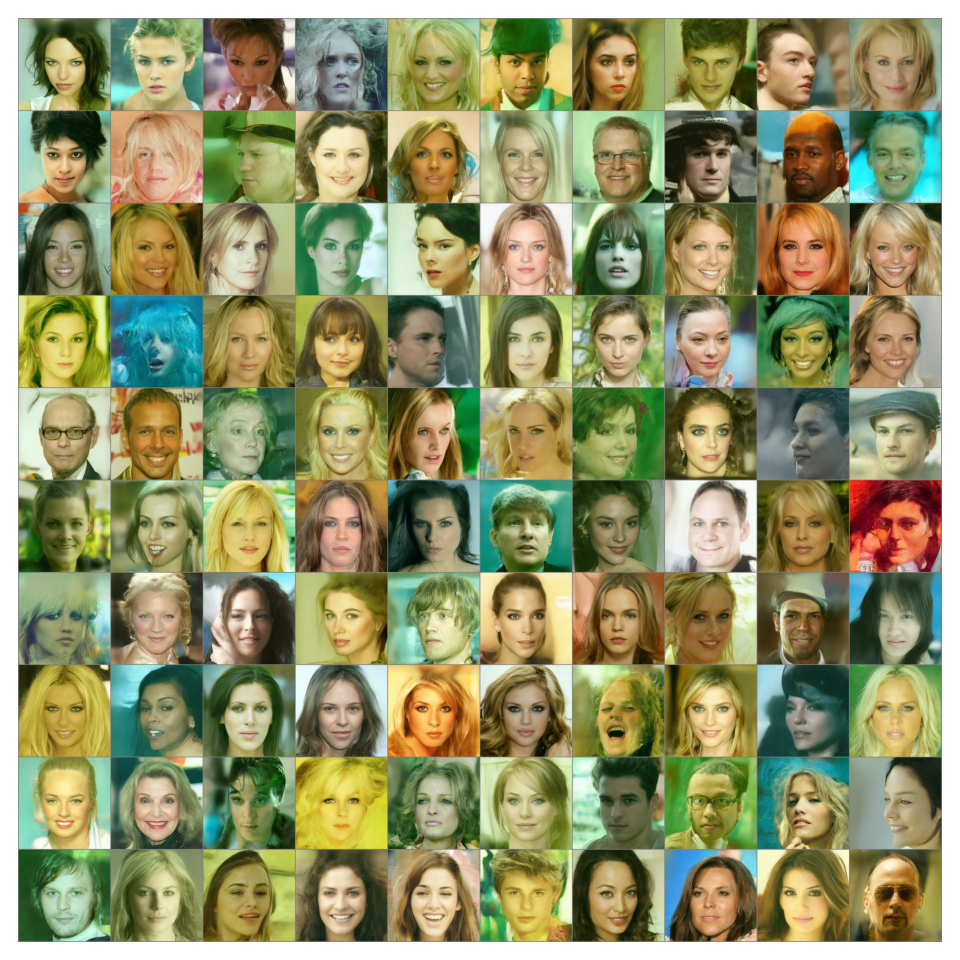
\includegraphics[scale=0.8]{img/results/ddpm-samples.png}
            \vspace{-4pt}  % reduce space between caption and figure
            \captionsetup{width=\textwidth} % set the width of the caption
            \caption{Celeba-HQ 256x256 generated samples from the pretrained model google/ddpm-celebahq-256.}
            \label{fig:ddpm-samples}
        \end{figure}

        % 100 samples from the finetuned model with ddpo and compressibility
        \begin{figure}
            \centering
            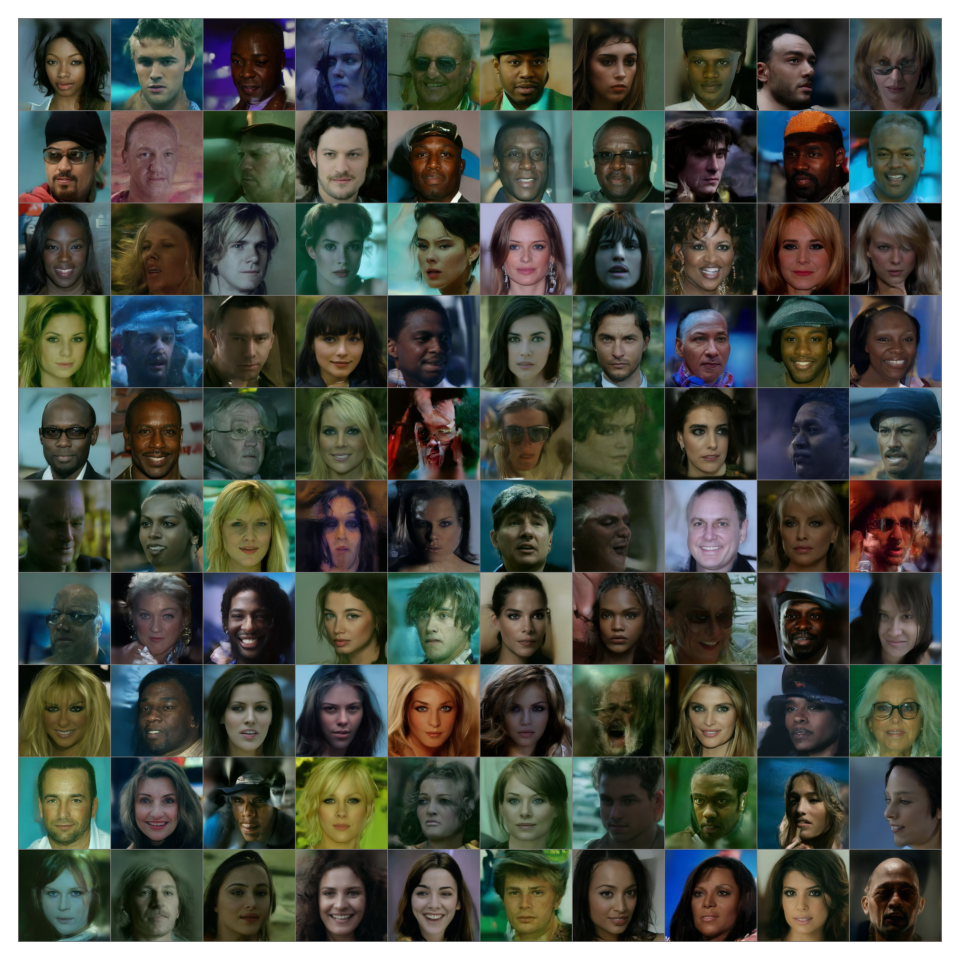
\includegraphics[scale=0.8]{img/results/ddpo-compressibility-samples.png}
            \vspace{-4pt}  % reduce space between caption and figure
            \captionsetup{width=\textwidth} % set the width of the caption
            \caption{Celeba-HQ 256x256 generated samples from the DDPO finetuned model optimized by JPEG compressibility.}
            \label{fig:ddpo-compressibility-samples}
        \end{figure}

        % 100 samples from the finetuned model with ddpo and incompressibility
        \begin{figure}
            \centering
            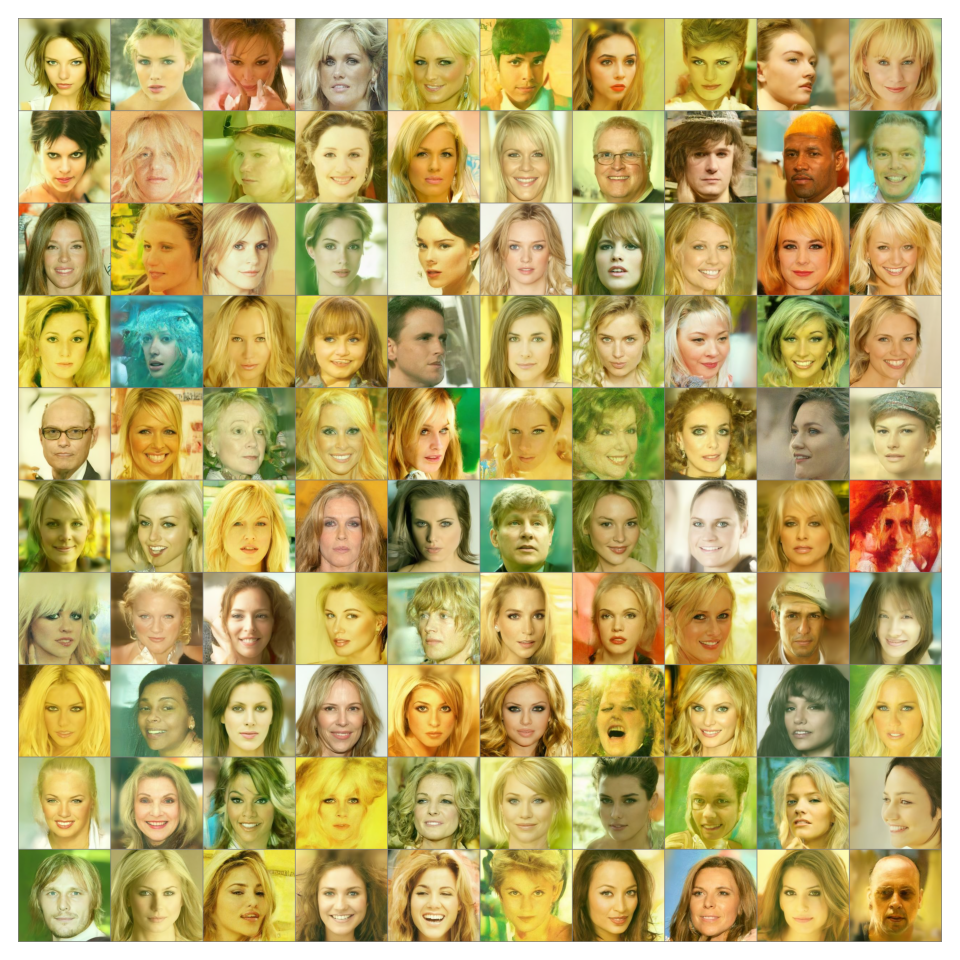
\includegraphics[scale=0.8]{img/results/ddpo-incompressibility-samples.png}
            \vspace{-4pt}  % reduce space between caption and figure
            \captionsetup{width=\textwidth} % set the width of the caption
            \caption{Celeba-HQ 256x256 generated samples from the DDPO finetuned model optimized by JPEG incompressibility.}
            \label{fig:ddpo-incompressibility-samples}
        \end{figure}

        % 100 samples from the finetuned model with ddpo and aesthetic quality
        \begin{figure}
            \centering
            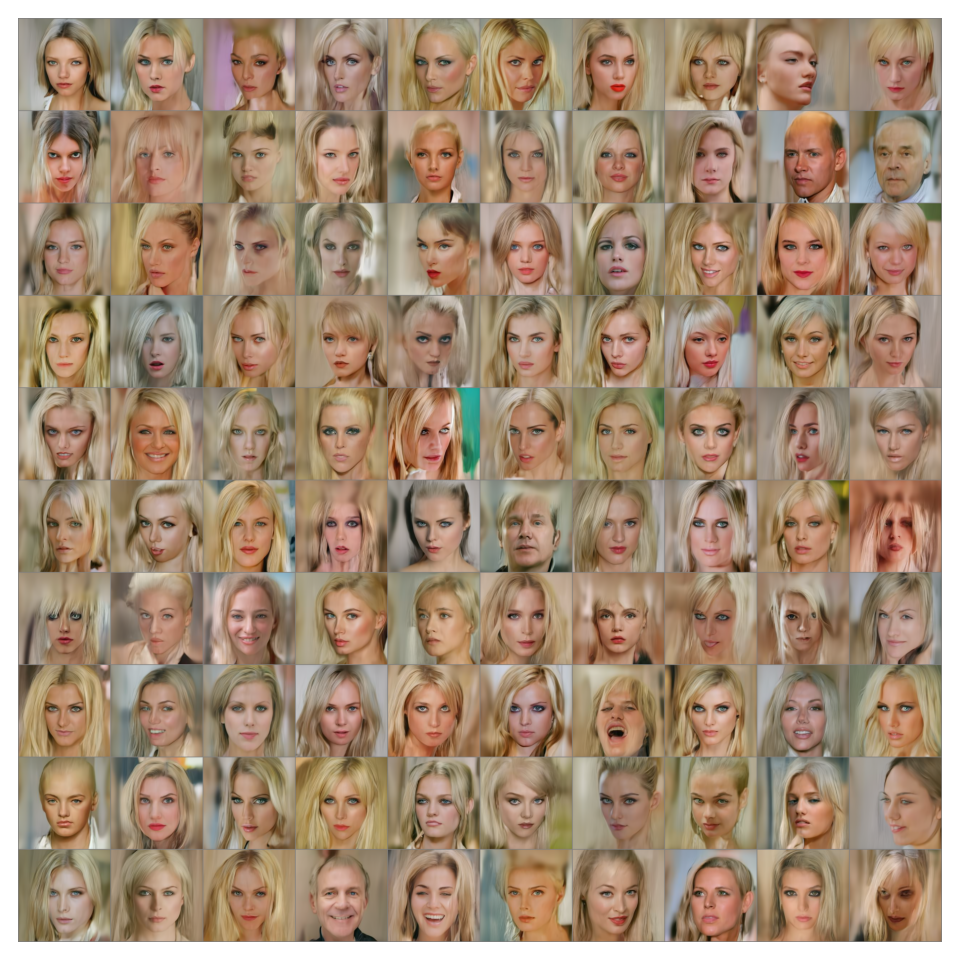
\includegraphics[scale=0.8]{img/results/ddpo-aesthetic-samples.png}
            \vspace{-4pt}  % reduce space between caption and figure
            \captionsetup{width=\textwidth} % set the width of the caption
            \caption{Celeba-HQ 256x256 generated samples from the DDPO finetuned model optimized by aesthetic quality.}
            \label{fig:ddpo-aesthetic-samples}
        \end{figure}

    \newpage

    \section{Additional transitions from DDPM to DDPO}

    \ca{Cambiar captions de las figuras de transición..., buscar una descripción más adecuada y también mejorar el caption de los ejemplos que aparecen en el capítulo de resultados.}

        % transition using jpeg compressibility extra sample 1
        \begin{figure}
            \centering
            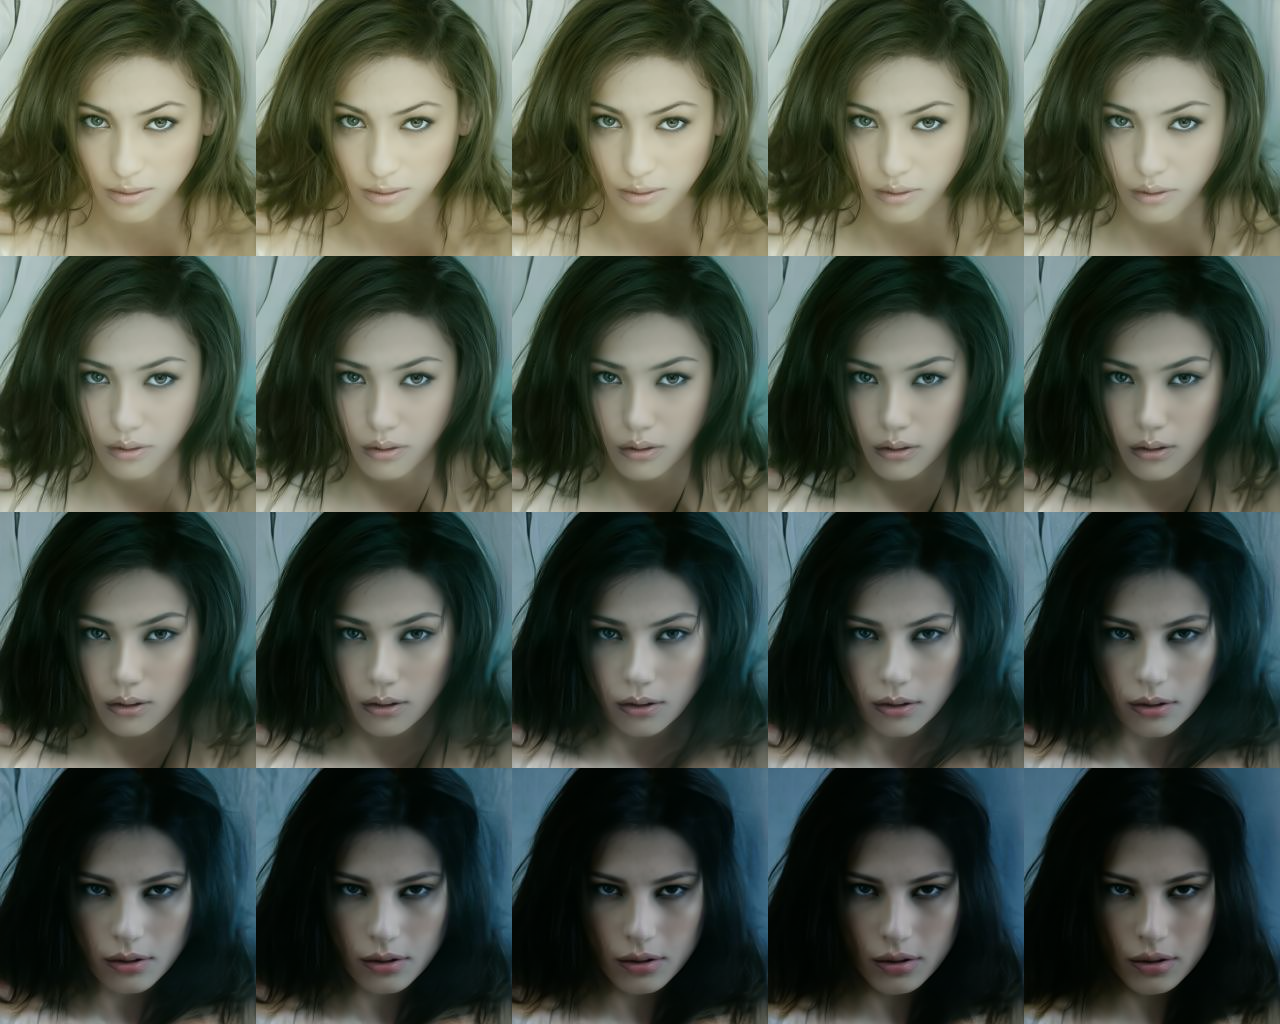
\includegraphics[scale=1.40]{img/results/compressibility_40.png}
            \vspace{-0pt}  % reduce space between caption and figure
            \captionsetup{width=\textwidth} % set the width of the caption
            \caption{Celeba-HQ 256x256 generated samples from the DDPO finetuned model optimized by JPEG compressibility.}
            \label{fig:ddpm-to-ddpo-compressibility-extra1}
        \end{figure}

        % transition using jpeg compressibility extra sample 2
        \begin{figure}
            \centering
            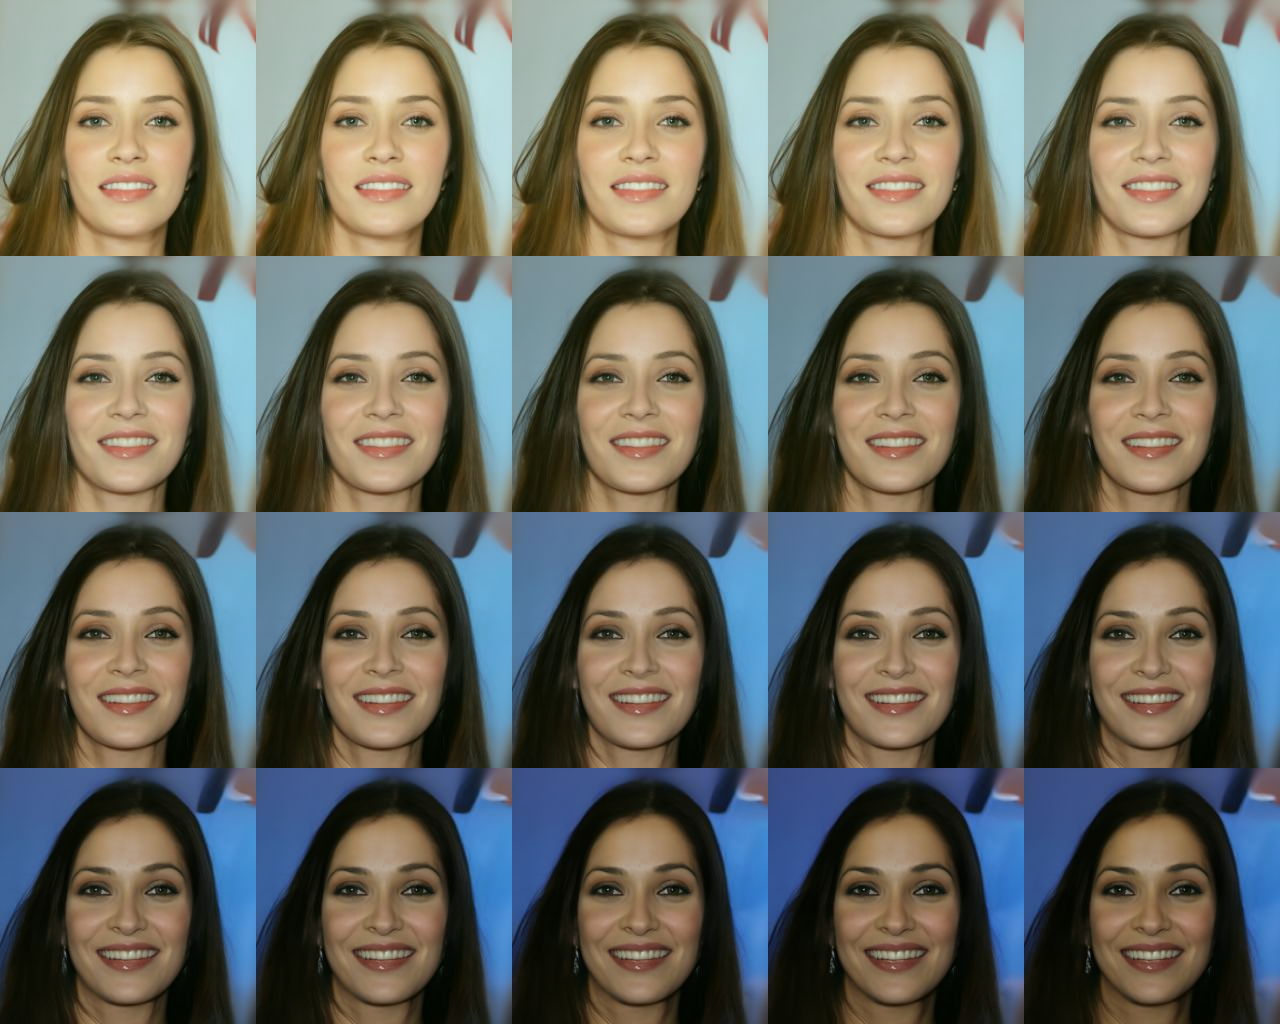
\includegraphics[scale=1.40]{img/results/compressibility_44.png}
            \vspace{-0pt}  % reduce space between caption and figure
            \captionsetup{width=\textwidth} % set the width of the caption
            \caption{Celeba-HQ 256x256 generated samples from the DDPO finetuned model optimized by JPEG compressibility.}
            \label{fig:ddpm-to-ddpo-compressibility-extra2}
        \end{figure}

        % transition using jpeg incompressibility extra sample 1
        \begin{figure}
            \centering
            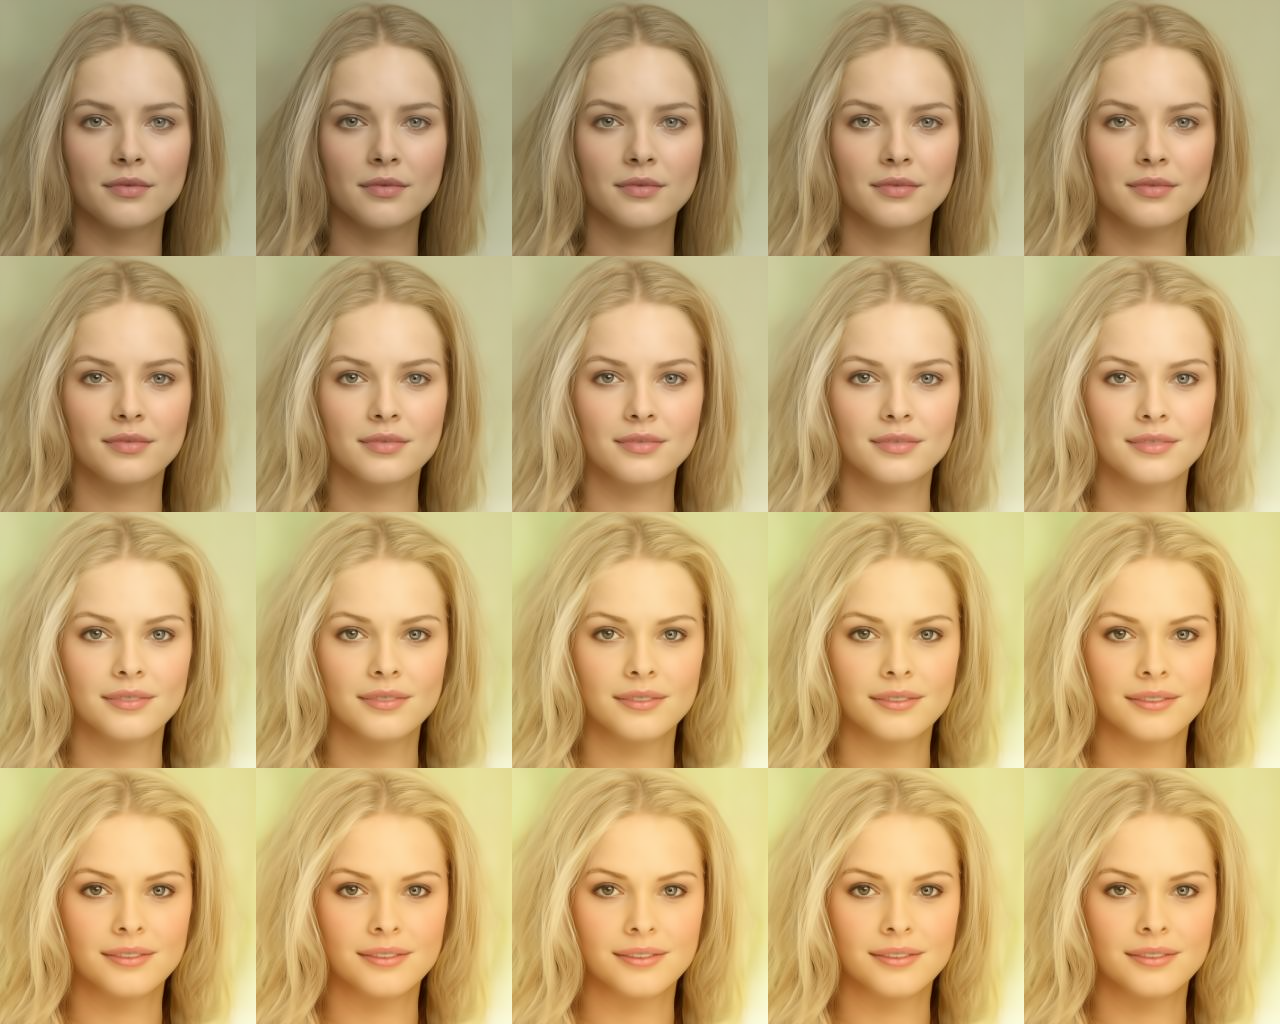
\includegraphics[scale=1.40]{img/results/incompressibility_8.png}
            \vspace{-0pt}  % reduce space between caption and figure
            \captionsetup{width=\textwidth} % set the width of the caption
            \caption{Celeba-HQ 256x256 generated samples from the DDPO finetuned model optimized by JPEG incompressibility.}
            \label{fig:ddpm-to-ddpo-incompressibility-extra1}
        \end{figure}


        % transition using jpeg incompressibility extra sample 2
        \begin{figure}
            \centering
            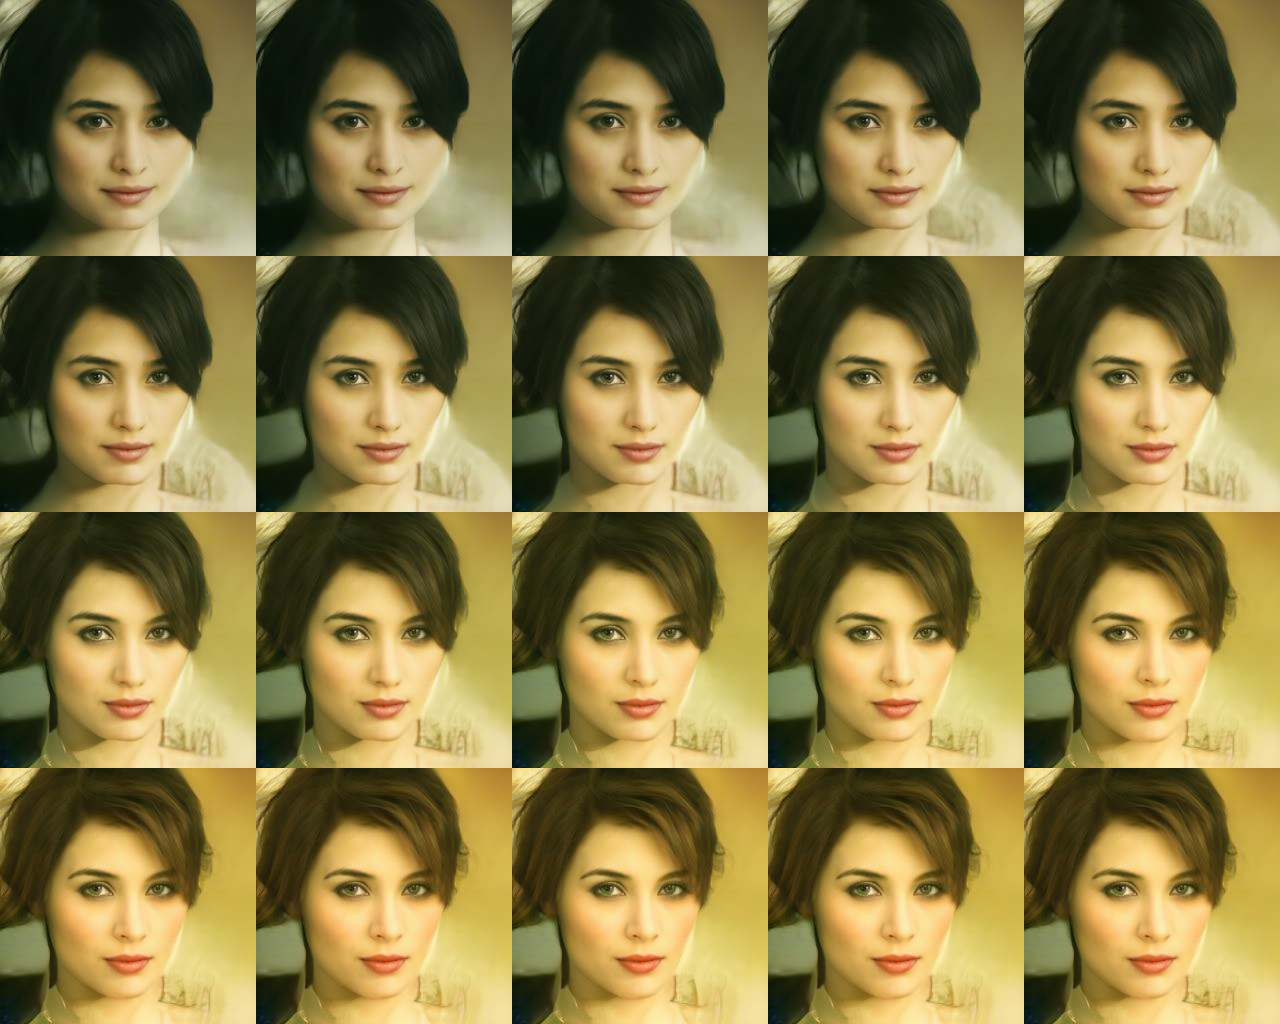
\includegraphics[scale=1.40]{img/results/incompressibility_28.png}
            \vspace{-0pt}  % reduce space between caption and figure
            \captionsetup{width=\textwidth} % set the width of the caption
            \caption{Celeba-HQ 256x256 generated samples from the DDPO finetuned model optimized by JPEG incompressibility.}
            \label{fig:ddpm-to-ddpo-incompressibility-extra2}
        \end{figure}

        % transition using aesthetic quality extra sample 1
        \begin{figure}
            \centering
            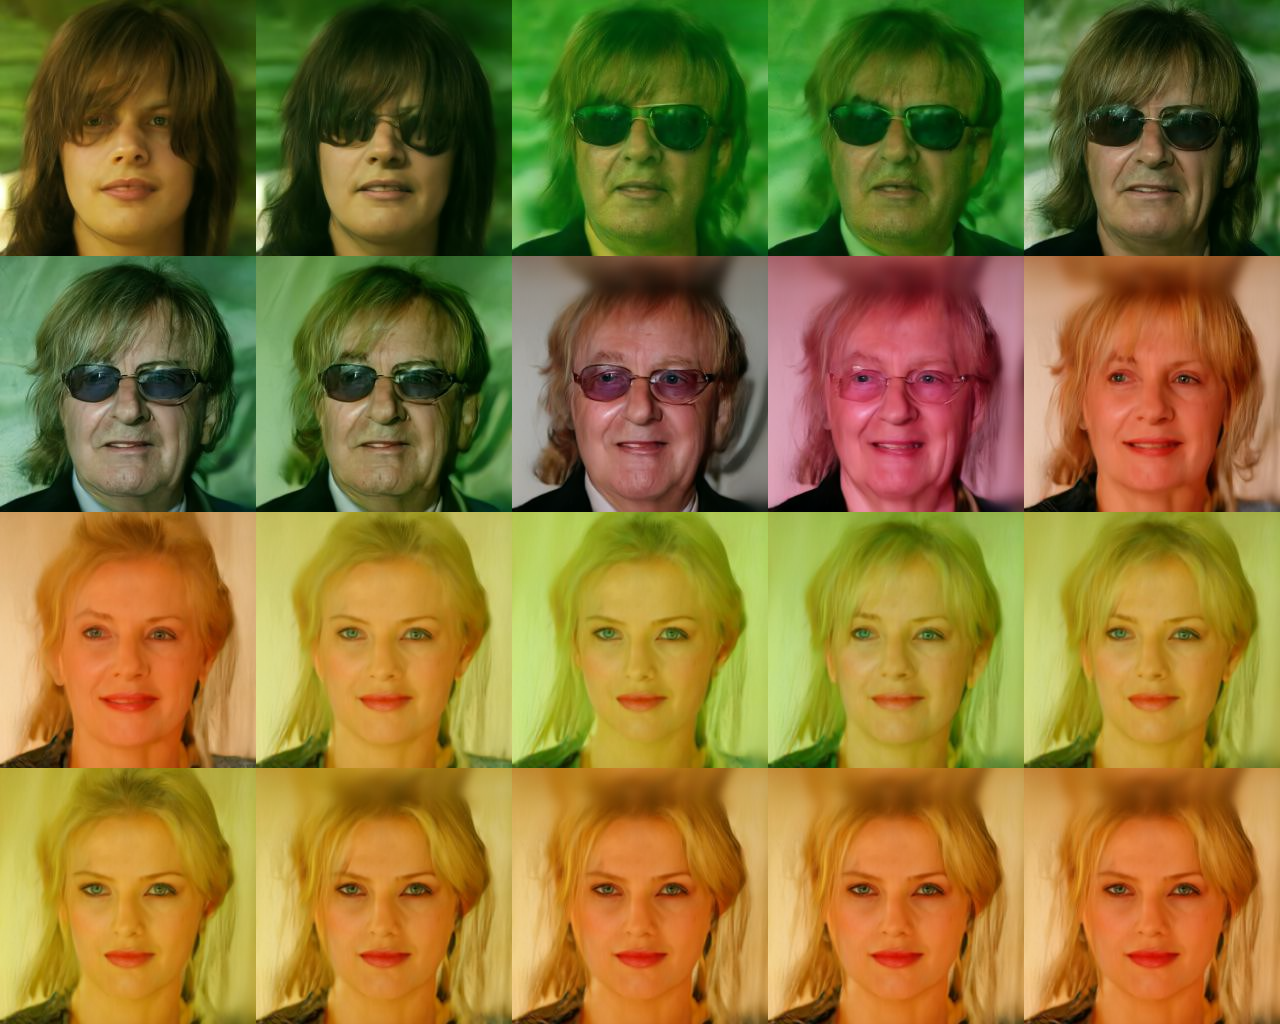
\includegraphics[scale=1.40]{img/results/laion_1.png}
            \vspace{-0pt}  % reduce space between caption and figure
            \captionsetup{width=\textwidth} % set the width of the caption
            \caption{Celeba-HQ 256x256 generated samples from the DDPO finetuned model optimized by aesthetic quality.}
            \label{fig:ddpm-to-ddpo-aesthetic-extra1}
        \end{figure}


        % transition using aesthetic quality extra sample 2
        \begin{figure}
            \centering
            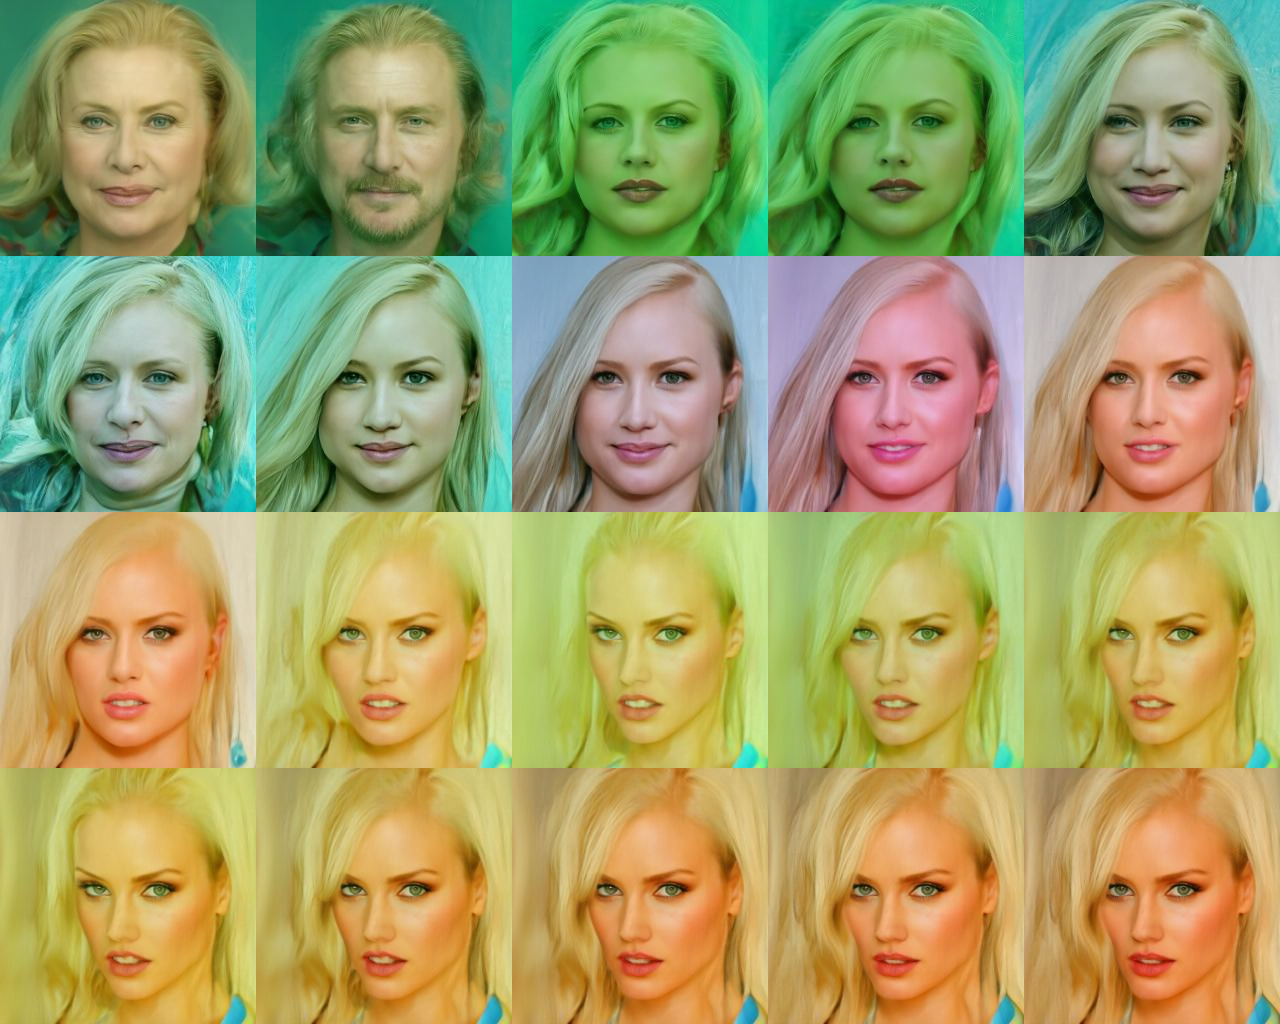
\includegraphics[scale=1.40]{img/results/laion_12.png}
            \vspace{-0pt}  % reduce space between caption and figure
            \captionsetup{width=\textwidth} % set the width of the caption
            \caption{Celeba-HQ 256x256 generated samples from the DDPO finetuned model optimized by aesthetic quality.}
            \label{fig:ddpm-to-ddpo-aesthetic-extra2}
        \end{figure}

        % transition from DDPM to DDPO samples optimized for Task.OVER50 (ViT age classifier) extra sample 1
        \begin{figure}
            \centering
            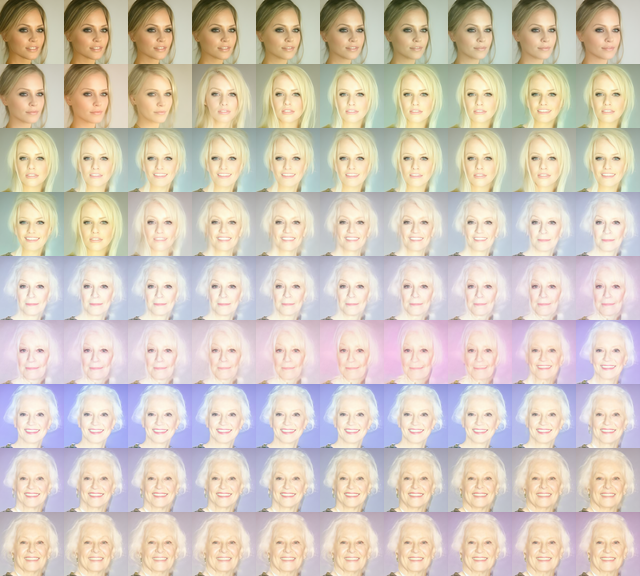
\includegraphics[scale=2.80]{img/results/over50_7.png}
            \vspace{-0pt}  % reduce space between caption and figure
            \captionsetup{width=\textwidth} % set the width of the caption
            \caption{Transition from DDPM to DDPO optimized for over50.}
            \label{fig:ddpm-to-ddpo-over50-extra1}
        \end{figure}

        % transition from DDPM to DDPO samples optimized for Task.OVER50 (ViT age classifier) extra sample 2
        \begin{figure}
            \centering
            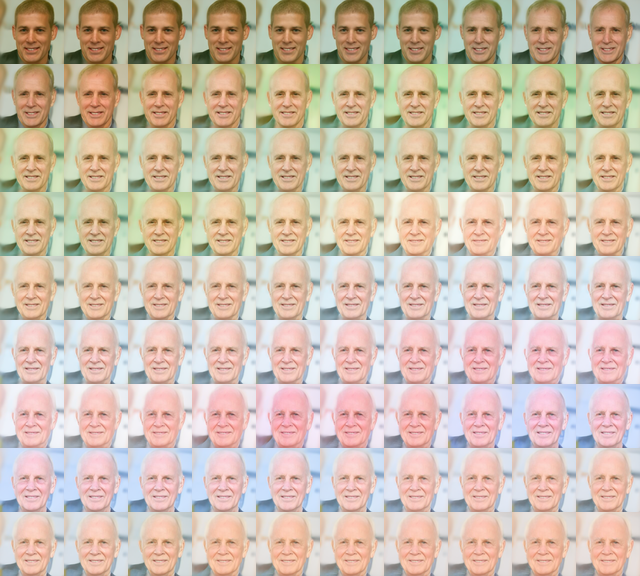
\includegraphics[scale=2.80]{img/results/over50_46.png}
            \vspace{-0pt}  % reduce space between caption and figure
            \captionsetup{width=\textwidth} % set the width of the caption
            \caption{Transition from DDPM to DDPO optimized for over50.}
            \label{fig:ddpm-to-ddpo-over50-extra2}
        \end{figure}


    \newpage

    \section{Implementation details}\label{appendix:implementation}

    The DDPO finetuned checkpoints are available in the following Hugging Face
    model repositories: \ca{Create a table with the model and the respective
    W\&B run (make public the project)}
    \begin{enumerate}
        \item \href{https://huggingface.co/alkzar90/ddpo-compressibility-celebahq-256}{alkzar90/ddpo-compressibility-celebahq-256}
        \item \href{https://huggingface.co/alkzar90/ddpo-incompressibility-celebahq-256}{alkzar90/ddpo-incompressibility-celebahq-256}
        \item \href{https://huggingface.co/alkzar90/ddpo-aesthetic-celebahq-256}{alkzar90/ddpo-aesthetic-celebahq-256}
    \end{enumerate}

    Mention the use of the Hugging Face diffuser library...

    \subsection{Hyperparameters}

    XYZ

	% Tablas
	\enabletablerowcolor[2] % Activa el color de celda
	\begin{table}[H]
		\begin{threeparttable}
		\centering
		\caption{Hyperparameters used in the experiments.}
		\begin{tabular}{cccC{4cm}}
			\hline
			\textbf{Elemento} & $\epsilon_i$ & \textbf{Valor} & \textbf{Descripción} \bigstrut \\
			\hline
			A     & 10    & 3,14$\pi$ & Valor muy interesante\tnote{a} \\
			B     & 20    & 6 & Segundo elemento \\
			C     & 30    & 7 & Tercer elemento\tnote{1} \\
			D     & 150    & 10 & Sin descripción \\
			E     & 0    & 0 & Cero \\
			\hline
			\end{tabular}
		\begin{tablenotes}
			\item[a] Este elemento tiene una descripción debajo de la tabla
			\item[1] Más comentarios
		\end{tablenotes}
		\end{threeparttable}
		\label{tab:anexo-1}
	\end{table}
	\disabletablerowcolor % Desactiva el color de celda

    \subsection{Linear Warmup \& Half-Cosine Decay}

    From the downstream task aesthetic quality the training dynamics present difficult to optimize the reward using a fixed learning rate. Improvement start to appears using...%The learning rate schedule is a linear warmup for the first 10\% of the training steps, followed by a half-cosine decay for the remaining 90\% of the training steps. The learning rate is multiplied by a factor of 0.1 at the end of the linear warmup and then decayed using a half-cosine decay schedule. The learning rate is initialized at $10^{-4}$ and the optimizer is Adam with $\beta_1 = 0.9$, $\beta_2 = 0.999$, and $\epsilon = 10^{-8}$.



\end{appendixs}